
\info{
	on rappelle les notations suivantes :

	\begin{itemize}
		\item vrai : $\theta = \mathds E \bigl[ \, f(X) \, \bigr]$
		\item intangible/inobservable : $\widetilde \theta = \frac 1 N \sum_i f(X_i)$
		\item observable : $\widehat \theta = \frac 1 N \sum_i f(\widehat X_i)$
	\end{itemize}
}

L'estimation des paramètres de régularité locale en $t_2$, $H_{t_2}$ et $L_{t_2}$, utilise les incréments quadratiques $\theta$ entre les différents points $t_1, t_2, t_3$ dans un voisinage de diamètre $\Delta$ autour de $t_2$.

\question{
	Quelle quantité est-il judicieux d'évaluer pour estimer au mieux la régularité locale en $t_2$ ? Doit-t-on regarder la qualité de l'approximation de $\theta$ (qui est une espérance) car il est utilisé pour tous les estimateurs ? Ou doit-on regarder la qualité de l'approximation de $H_{t_2}$ et $L_{t_2}$ car ce sont les quantités qui nous intéressent ? Ou bien les deux ?
}

Le choix du bon critère d'évaluation est d'une grande importance. Il faut se rappeler l'objectif que l'on cherche à atteindre : déterminer une procédure (simple si possible) de détermination de l'hyper-paramètre $\Delta$ utilisé pour l'estimation de la régularité locale en fonction de quantités facilement estimables, ou directement observables par le praticien. En observant que $L$ est estimée par une expression impliquant $\theta$ et $\Delta^{2 H}$, une estimation précise de $H$ paraît plus cruciale pour la bonne estimation des deux quantités. Bien qu'il existe certainement un compromis entre la bonne estimation de $H$ et de $L$ qui fournit une meilleure estimation adaptative des quantités qui nous intéressent, il est certainement plus probable de dériver une procédure de sélection de $\Delta$ simple à implémenter pour le praticien en se basant sur la qualité de l'estimation d'une unique quantité.

\question{
	Doit-t-on se concentrer sur l'estimation de $H$ ou de $\theta$ ?
}

Les incréments sont des quantités importantes dans l'estimation de la régularité, utilisées à la fois pour l'estimation de $H$ et de $L$, l'approche que l'on considère se base sur cette remarque. Nous allons donc chercher à déterminer un $\Delta$ adapté à l'estimation des incréments quadratiques. Toutefois, il y a plusieurs possibilités de $u,v \in J_\Delta(t_2)$ que l'on peut considérer pour l'estimation de $H$ et $L$. C'est pourquoi nous décidons de considérer les \emph{couples} d'incréments utilisés pour l'estimation de $H$. Ainsi en posant :

\begin{minipage}{0.5\textwidth}
	\begin{equation*}
		\thetaA = \begin{bmatrix} \theta(t_1, t_3) \\ \theta(t_1, t_2) \end{bmatrix}
	\end{equation*}
\end{minipage}
\hfill
\begin{minipage}{0.5\textwidth}
	\begin{equation*}
		\thetaB = \begin{bmatrix} \theta(t_1, t_3) \\ \theta(t_2, t_3) \end{bmatrix}
	\end{equation*}
\end{minipage}

\smallskip

L'estimateur du paramètre de régularité $H_t$ peut se ré-écrire comme :

\smallskip


\begin{equation*}
	\widehat H_t : \Theta = \begin{bmatrix} \Theta_1 \\ \Theta_2 \end{bmatrix} \longmapsto \frac{ \log \widehat \Theta_1 - \log \widehat \Theta_2 }{2 \log 2}
\end{equation*}

\smallskip

Le problème c'est qu'on ne dispose pas de la véritable valeur de $\theta(u,v)$, on pourrait exploiter le fait que l'on dipose d'un mouvement brownien multi-fractionnaire qui a été étudié de façon extensive dans la littérature, mais on décide de ne pas l'utiliser pour adopter une approche plus proche d'un cadre général.
Le meilleur estimateur que l'on puisse espérer atteindre est $\bigl(\hat H_t( \widetilde \thetaA)$ ou $\hat H_t( \widetilde \thetaB)\bigr)$, estimateur utilisant les courbes pleinement observées et non bruitées. On va donc s'intéresser désormais à l'erreur d'estimation conjointe des deux $\theta(u,v)$ utilisés dans l'estimation de $H_t$ par rapport à cet estimateur en quelque sorte \og idéal \fg de $\theta$ comme critère de sélection du diamètre $\Delta$.

\begin{figure}[H]
	\centering
	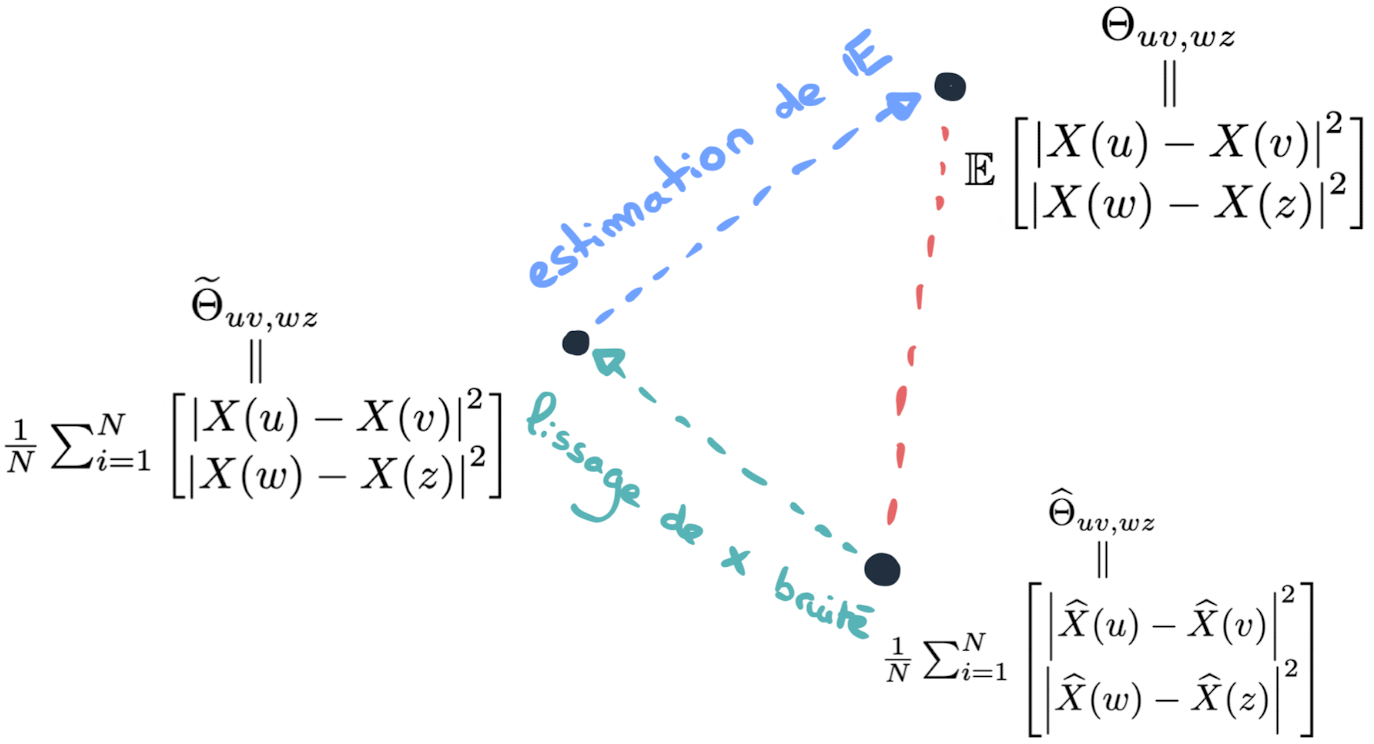
\includegraphics[width=0.7\textwidth]{Images/sketches/theta_biais.png}
	\caption{Schéma représentant les différentes approximations du couple d'incréments}
	\label{fig:sketch_theta_biais}
\end{figure}


Pour cela on considère la distance euclidienne usuelle pour des vecteurs de $\R 2$

$$R(\Theta, \Delta) = \distnorme 2 {\widehat \Theta(\Delta)} {\widetilde \Theta(\Delta)}$$

et on nomme $R\cindexA(\Delta) = R( \thetaA , \, \Delta \, )$ et $R\cindexB(\Delta) = R( \thetaB, \, \Delta \, )$

\begin{table}[H]
	\centering
	\begin{tabular}{l|ll|}
		\cline{2-3}
		                                     & $\lambda < 120$                                                                                                                                                                                                           & $\lambda \geq 120$                                                                             \\ \hline
		\multicolumn{1}{|l|}{$H_t < 0.6$}    & \multicolumn{1}{l|}{\begin{tabular}[c]{@{}l@{}}$\yesequiv \mathcal R, \Delta^*$\\ $\Delta^*_- = 0.01$\end{tabular}}                                                                                                       & \begin{tabular}[c]{@{}l@{}}$\thetaB$\\ $\Delta^*_+ = 0.2$\end{tabular}                         \\ \cline{2-3}
		\multicolumn{1}{|l|}{$H_t \geq 0.6$} & \multicolumn{1}{l|}{\begin{tabular}[c]{@{}l@{}}$\thetaB$\\ $\Delta^*_- = 0.2$\\ \\\faExclamationTriangle $H=0.7 : \Delta^- = 0.01 \oplus \yesequiv \mathcal R$\\ \\\faExclamationTriangle $H=0.8 : \thetaA$\end{tabular}} & \begin{tabular}[c]{@{}l@{}}$\yesequiv \mathcal R, \Delta^*$\\ $\Delta^*_+ = 0.01$\end{tabular} \\ \hline
	\end{tabular}
	\label{tab:recap_delta_eucl_h_global_pour_lambda_sup}
	\caption{Tableau récapitulatif des $\Delta$ optimaux : Risque euclidien sur $\tilde \Theta$ | fenêtre de prélissage globale pour $\lambda \geq 120$}
\end{table}
